\documentclass[11pt,a4paper]{article}

\usepackage[utf8]{inputenc}
\usepackage[T1]{fontenc}
\usepackage[italian]{babel}
\usepackage[margin=2.1cm, top=2.2cm, bottom=2.2cm]{geometry}
\usepackage{amsmath,amssymb}
\usepackage{graphicx}
\usepackage{booktabs}
\usepackage{tabularx}
\usepackage{array}
\usepackage{xcolor}
\usepackage{listings}
\usepackage{fancyhdr}
\usepackage{titlesec}
\usepackage{enumitem}
\usepackage{hyperref}

\definecolor{accentBlue}{HTML}{1D4ED8}
\definecolor{darkSlate}{HTML}{1E293B}
\definecolor{checkGreen}{HTML}{15803D}
\definecolor{codeBg}{HTML}{F8FAFC}
\definecolor{codeBorder}{HTML}{CBD5E1}

\hypersetup{
    colorlinks=true,
    linkcolor=accentBlue,
    urlcolor=accentBlue,
    pdftitle={Astro-Miner 2D: Cosmic Coin Rush - Relazione Tecnica},
    pdfauthor={Arianna Palmucci}
}

\pagestyle{fancy}
\fancyhf{}
\lhead{\small\textcolor{darkSlate}{Astro-Miner 2D: Cosmic Coin Rush}}
\rhead{\small\textcolor{darkSlate}{Elaborato 1 -- Computer Graphics (UniBo)}}
\cfoot{\small\thepage}
\renewcommand{\headrulewidth}{0.4pt}

\titleformat{\section}{\large\bfseries\color{accentBlue}}{\thesection.}{0.5em}{}
\titleformat{\subsection}{\normalsize\bfseries\color{darkSlate}}{\thesubsection}{0.5em}{}
\titlespacing*{\section}{0pt}{13pt}{5pt}
\titlespacing*{\subsection}{0pt}{9pt}{4pt}
\setlist[itemize]{itemsep=3pt, topsep=4pt, leftmargin=1.4em}

\lstset{
    basicstyle=\ttfamily\footnotesize,
    backgroundcolor=\color{codeBg},
    frame=single,
    rulecolor=\color{codeBorder},
    breaklines=true,
    showstringspaces=false,
    tabsize=4,
    aboveskip=7pt,
    belowskip=7pt
}

\begin{document}

% ==============================================================================
% INTESTAZIONE
% ==============================================================================
\begin{center}
    {\LARGE\bfseries\color{darkSlate} Astro-Miner 2D: Cosmic Coin Rush}\\[5pt]
    {\normalsize\color{accentBlue} Relazione Tecnica -- Elaborato 1 di Computer Graphics}\\[8pt]
    {\small\textbf{Candidata:} Arianna Palmucci \quad|\quad \textbf{Docente:} Prof.ssa Damiana Lazzaro \quad|\quad \textbf{A.A.} 2026/2027}\\
    {\small\textbf{Tecnologie:} C++17, OpenGL 3.3 Core Profile, GLSL (\texttt{\#version 330 core}), GLFW, GLAD, GLM, Dear ImGui, \texttt{stb\_image}}
\end{center}
\vspace{4pt}
\hrule
\vspace{10pt}

\noindent\textbf{Panoramica.} \textit{Astro-Miner 2D: Cosmic Coin Rush} è un ambiente grafico e videogioco arcade 2D interattivo sviluppato in C++17 e OpenGL 3.3 Core Profile. Il giocatore pilota una navicella mineraria per raccogliere 5 monete cosmiche evitando asteroidi, dardi di plasma perimetrali e un drone sentinella, fino ad attivare e attraversare il portale \textit{Warp Gate}. Il progetto adotta un'architettura modulare priva di variabili globali esposte, con gestione automatica delle risorse GPU tramite \textbf{RAII} e \textbf{Rule of Five} (copia vietata sugli handle OpenGL, semantica di movimento abilitata).

% ==============================================================================
\section{Architettura Software, Pipeline OpenGL e Game Loop}
% ==============================================================================
Il motore applica la \textit{Separation of Concerns} suddividendo il codice in quattro livelli indipendenti:

\begin{center}
\small
\begin{tabularx}{\linewidth}{@{}p{3.3cm} X@{}}
\toprule
\textbf{Livello} & \textbf{Moduli e Responsabilità} \\
\midrule
\textbf{Core \& Input} & \texttt{main.cpp} (contesto OpenGL 3.3 Core Profile, GLAD, alpha blending, Dear ImGui, render loop), \texttt{Input} (callback tastiera \texttt{ESC}, resize \texttt{glViewport}, inversione asse $Y$ del cursore rispetto all'origine in basso a sinistra di OpenGL). \\
\textbf{Orchestrazione} & \texttt{GameWorld} (pattern \textbf{Facade} verso \texttt{main.cpp} e \textbf{FSM} a tre stati: \texttt{PLAYING}, \texttt{LEVEL\_CLEARED\_HURRA}, \texttt{GAME\_OVER}). \\
\textbf{Layer GPU} & \texttt{MeshData}, \texttt{ShapeGenerator}, \texttt{Geometry} (VAO/VBO RAII), \texttt{Shader}, \texttt{ShaderMaker} (compilazione e linking GLSL a runtime), \texttt{Texture} (\texttt{stb\_image}), \texttt{Transform}. \\
\textbf{Scena \& Fisica} & \texttt{BackgroundRenderer}, \texttt{Player}, \texttt{PlayerShapeLoader}, \texttt{AsteroidManager}, \texttt{CollectibleManager}, \texttt{HermiteManager}, \texttt{LaserManager}, \texttt{HazardManager}, \texttt{ParticleSystem}, \texttt{Collider2D}. \\
\bottomrule
\end{tabularx}
\end{center}

\begin{sloppypar}
\noindent\textbf{Origine dei moduli:} \texttt{ShaderMaker} riprende quasi integralmente la base dei laboratori del corso; \texttt{ShapeGenerator}, \texttt{Geometry}, \texttt{Shader}, \texttt{Texture}, \texttt{MeshData}, \texttt{Transform}, \texttt{Input}, \texttt{HermiteObject} e lo scheletro GLFW/GLAD/ImGui di \texttt{main.cpp} adattano i pattern di laboratorio in classi C++ RAII; tutti i restanti manager di gioco e di rendering (\texttt{GameWorld}, \texttt{Player}, \texttt{PlayerShapeLoader}, \texttt{AsteroidManager}, \texttt{CollectibleManager}, \texttt{LaserManager}, \texttt{HazardManager}, \texttt{ParticleSystem}, \texttt{BackgroundRenderer}, \texttt{Collider2D}, \texttt{MathConstants}) sono progettati ex novo.
\end{sloppypar}

\subsection{Inizializzazione, Delta Time e Visibilità senza Depth Test}
In \texttt{main.cpp}, la richiesta di \texttt{GLFW\_OPENGL\_CORE\_PROFILE} (con \texttt{GLFW\_OPENGL\_FORWARD\_COMPAT} su macOS) esclude la pipeline fissa deprecata (\texttt{glBegin}/\texttt{glEnd}/\texttt{glMatrixMode}), imponendo l'uso esplicito di VAO, VBO e shader GLSL. Ogni iterazione del game loop misura il passo temporale $\Delta t = t_{\text{corr}} - t_{\text{prec}}$ tramite \texttt{glfwGetTime()} e applica il \textbf{Delta-Time Clamping}:
\[
\Delta t_{\text{eff}} = \min(\Delta t,\, 0.05\,\text{s})
\]
In tal modo cinematica, rotazioni, timer di invulnerabilità e particelle restano indipendenti dal refresh rate del monitor (60~Hz o 120~Hz), prevenendo errori di \textit{tunneling} in caso di pausa o lag. Poiché tutte le geometrie giacciono sul piano $z=0$ e fanno ampio uso di trasparenze, \texttt{GL\_DEPTH\_TEST} rimane disabilitato per evitare \textit{Z-fighting} e occlusioni errate sulle particelle; la visibilità è gestita dall'ordine rigoroso \textbf{Back-to-Front} in \texttt{GameWorld::render}:
\[
\text{Sfondo (NDC)} \longrightarrow \text{Oggetti solidi} \longrightarrow \text{Navicella + Ritratto} \longrightarrow \text{Fiamme, LED, Particelle \& UI}
\]

% ==============================================================================
\section{Modellazione Gerarchica, Texture e Curve di Hermite}
% ==============================================================================
\subsection{Navicella Composita e Simmetria Speculare (Requisito 3.1)}
In \texttt{Player.cpp}, la navicella è assemblata come albero di trasformazione gerarchica in coordinate omogenee $4\times 4$ (necessarie sia per esprimere la traslazione tramite prodotto matriciale, sia per allinearsi allo spazio clip 4D di OpenGL). La matrice radice porta il frame locale nella posa globale:
\[
\mathbf{M}_{\text{player}} = \mathbf{T}(p_x, p_y) \cdot \mathbf{R}_z(\theta - 90^\circ)
\]
Ogni sotto-componente (fusoliera trapezoidale, muso triangolare, cabina ellittica con riflesso, ali a delta, doppi cannoni, ugelli, fiamme reattive e LED verde/rosso) parte da \texttt{playerRoot} e applica $\mathbf{M}_{\text{comp}} = \mathbf{M}_{\text{player}} \cdot \mathbf{M}_{\text{locale}}$, muovendosi e ruotando solidalmente con la navicella. Per l'ala e il cannone di sinistra si evita la duplicazione dei vertici in VRAM specchiando la mesh destra con scala orizzontale negativa $\mathbf{S}(-1, 1, 1)$:
\begin{lstlisting}[language=C++]
for (float side : { 1.0f, -1.0f }) {
    glm::mat4 wingMat = glm::translate(playerRoot, glm::vec3(18.0f * side, -6.0f, 0.0f));
    wingMat = glm::scale(wingMat, glm::vec3(26.0f * side, 32.0f, 1.0f));
    shader.setMat4("model", wingMat);
    m_wingsGeo.draw();
}
\end{lstlisting}

\subsection{Texture Mapping e Ritratto Ellittico nel Cockpit}
Sul cupolino è proiettato un quad da 6 vertici con attributi interleaved $(x, y, z, u, v)$ la cui immagine è caricata da \texttt{Texture::load()}. Poiché le immagini su disco hanno origine in alto a sinistra mentre OpenGL colloca $(0,0)$ in basso a sinistra, viene invocato \texttt{stbi\_set\_flip\_vertically\_on\_load(1)} prima di \texttt{glTexImage2D}, con filtro bilineare \texttt{GL\_LINEAR} e clamping \texttt{GL\_CLAMP\_TO\_EDGE}. Il fragment shader \texttt{texture.frag} esegue una mascheratura analitica con bordo morbido:
\begin{lstlisting}[language=C++]
vec2 uvNorm = (vTexCoord - vec2(0.5, 0.5)) * 2.0;
float dist = dot(uvNorm, uvNorm);
if (dist > 1.0) discard;
vec4 texColor = texture(uTexture, vTexCoord);
float edgeAlpha = smoothstep(1.0, 0.82, dist);
FragColor = vec4(texColor.rgb, texColor.a * edgeAlpha) * uColorTint;
\end{lstlisting}

\subsection{Spline Cubiche di Hermite e Orbita di Lissajous (Requisito 3.2)}
Le due geometrie curvilinee avanzate (\texttt{alien\_drone.obj}, 113 vertici e 112 triangoli; \texttt{warp\_gate.obj}, 144 vertici e 144 triangoli) sono modellate tramite spline cubiche interpolanti di Hermite su $[0, 1]$:
\[
\mathbf{C}(t) = h_{00}(t)\mathbf{P}_0 + h_{01}(t)\mathbf{P}_1 + h_{10}(t)\mathbf{D}_0 + h_{11}(t)\mathbf{D}_1
\]
dove $h_{00}(t)=2t^3-3t^2+1$, $h_{01}(t)=-2t^3+3t^2$, $h_{10}(t)=t^3-2t^2+t$, $h_{11}(t)=t^3-t^2$. Nei nodi interni viene garantita la continuità parametrica $C^1$ (uguaglianza di posizione e di vettore tangente derivata $\mathbf{C}'_{i-1}(1)=\mathbf{C}'_i(0)$). I file OBJ/MTL (contenenti solo posizioni e colore piatto \texttt{Kd}, senza modelli di illuminazione 3D) sono caricati a runtime da \texttt{PlayerShapeLoader}.
\begin{itemize}
    \item \textbf{Alien Sentinel Drone:} testa cornuta con tratti del viso gerarchici (occhio circolare, pupilla rettangolare, sopracciglia e bocca). Pattuglia lungo una curva chiusa e regolare $C^1$ di \textbf{Lissajous}:
    \[
    x(\phi) = 640 + 340\cos(\phi), \qquad y(\phi) = 380 + 160\sin(2\phi)
    \]
    Quando la navicella lo sorvola esegue un ammiccamento (\textit{eye-blink}); se colpito dal laser si indebolisce per $4.5\,\text{s}$ diventando innocuo.
    \item \textbf{Cosmic Warp Gate:} anello cavo con vortice interno rotante che si attiva alla raccolta di tutte e 5 le monete.
\end{itemize}

% ==============================================================================
\section{Buffer Sharing, Pipeline Shader e Sfondo Procedurale}
% ==============================================================================
\subsection{Buffer Statici GPU e Istanziazione Multipla (Requisito 4)}
\texttt{ShapeGenerator} prepara le geometrie su CPU dentro \texttt{MeshData} (\texttt{positions}, \texttt{colors}, \texttt{primitiveType}) usando primitive \texttt{GL\_TRIANGLES} e \texttt{GL\_TRIANGLE\_FAN} in coordinate polari. \texttt{Geometry::upload()} crea un VAO (che registra il formato degli attributi \texttt{location 0} e \texttt{1}) e due VBO caricati in VRAM una sola volta con \texttt{GL\_STATIC\_DRAW}. Per asteroidi e monete viene applicato il \textbf{Buffer Sharing}:
\begin{lstlisting}[language=C++]
for (const auto& a : m_asteroids) {
    if (a.active) {
        glm::mat4 m = glm::translate(glm::mat4(1.0f), glm::vec3(a.pos, 0.0f));
        m = glm::rotate(m, glm::radians(a.rotation), glm::vec3(0, 0, 1));
        m = glm::scale(m, glm::vec3(a.scale, a.scale, 1.0f));
        shader.setMat4("model", m);
        m_asteroidGeo.draw(); // Riusa lo stesso VAO/VBO senza ricaricare vertici
    }
}
\end{lstlisting}
Le 5 monete d'oro (36 spicchi \texttt{GL\_TRIANGLES} con gradiente radiale giallo--ambra interpolato dalla GPU tramite coordinate baricentriche) levitano in $Y$ e simulano una rotazione pseudo-3D modulando la scala orizzontale con $|\cos(\omega t)|$.

\subsection{Shader Program Dedicati (Requisito 5)}
Gli shader sono compilati e linkati a runtime da \texttt{ShaderMaker}. A differenza di \texttt{basic.vert} e \texttt{texture.vert}, che applicano la proiezione ortografica \texttt{glm::ortho(0, 1280, 0, 720, -1, 1)}, lo shader dello sfondo (\texttt{BackgroundRenderer}) disegna un quad fullscreen già espresso in \textbf{NDC $[-1, 1]$} senza matrici \texttt{model} o \texttt{projection}:

\begin{center}
\small
\begin{tabularx}{\linewidth}{@{}l l X@{}}
\toprule
\textbf{Shader GLSL} & \textbf{Spazio} & \textbf{Funzionalità Principale} \\
\midrule
\texttt{background.vert/.frag} & NDC $[-1,1]$ & Nessuna texture: coordinate polari, spirale, \textit{domain warping} modulato da \texttt{uPsychedelic}, alternanza palette per \texttt{uLevel}, vignettatura e 3 layer stellari (\texttt{hash}, \texttt{smoothstep}, \texttt{sin(uTime)}). \\
\texttt{basic.vert/.frag} & \texttt{ortho * model} & Trasformazione 2D, interpolazione Gouraud di \texttt{vColor} e modulazione dinamica \texttt{uColorTint} per flash di danno e dissolvenze. \\
\texttt{texture.vert/.frag} & \texttt{ortho * model} & Campionamento texture pilota via \texttt{vTexCoord}, maschera ellittica (\texttt{discard}) e anti-aliasing sui bordi. \\
\bottomrule
\end{tabularx}
\end{center}

\noindent In \texttt{background.frag}, il campo stellare a tre strati di parallasse e la nebulosa fluida sono calcolati per ogni pixel su GPU senza alcuna lookup table esterna:
\begin{lstlisting}[language=C++]
float hash(vec2 p) {
    p = fract(p * vec2(123.34, 456.21));
    p += dot(p, p + 45.32);
    return fract(p.x * p.y);
}
\end{lstlisting}

\begin{figure}[htbp]
    \centering
    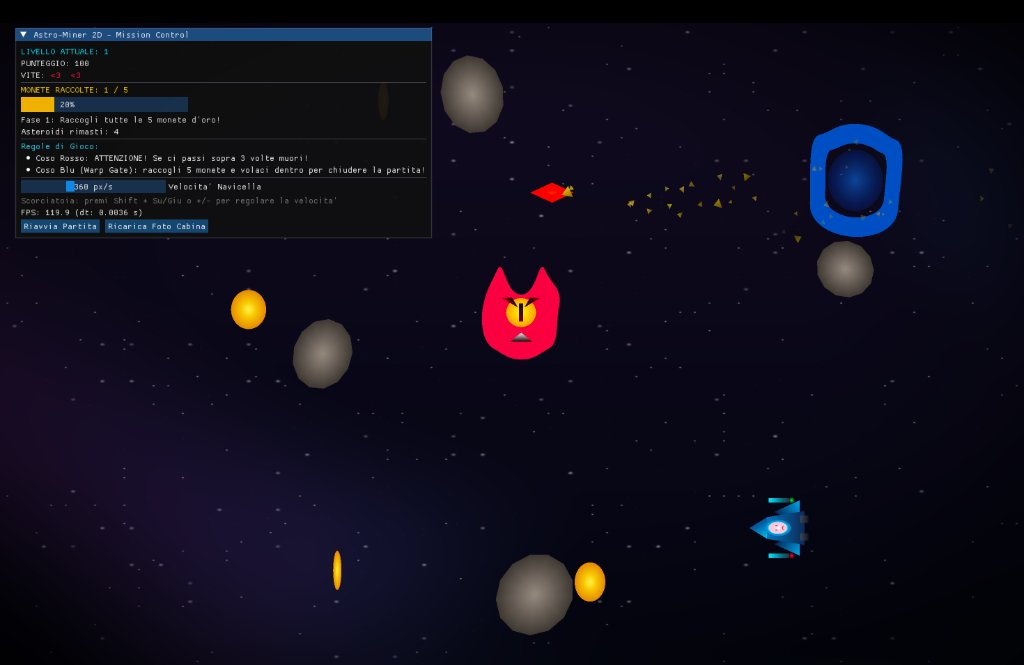
\includegraphics[width=0.76\linewidth]{../../assets/screenshots/screenshot_gameplay.jpg}
    \caption{Scena di gioco attiva: navicella gerarchica, Drone Rosso di Hermite, monete d'oro, asteroidi a buffer condiviso, Warp Gate, sfondo procedurale e HUD Dear ImGui.}
\end{figure}

% ==============================================================================
\section{Collisioni, Fisica Particellare, Interazione e Portabilità}
% ==============================================================================
\subsection{Collisioni Geometriche e Fisica delle Particelle}
\begin{itemize}
    \item \textbf{Collisioni (\texttt{Collider2D.h}):} il test \textit{Cerchio--Cerchio} confronta le distanze al quadrato ($\|\mathbf{c}_1-\mathbf{c}_2\|^2 \le (r_1+r_2)^2$) tramite \texttt{glm::dot}, evitando il calcolo della radice quadrata; il test \textit{Cerchio--AABB} applica il \textit{clamping} del centro sui limiti del rettangolo per trovare il punto più vicino.
    \item \textbf{Fisica Particellare e Alpha Blending (\texttt{ParticleSystem}):} alla distruzione di un asteroide vengono generati 32 frammenti (135 coriandoli alla vittoria), aggiornati con integrazione di Eulero e attrito viscoso lineare:
\end{itemize}
\begin{lstlisting}[language=C++]
p.pos += p.vel * dt;                  // Integrazione di Eulero
p.vel *= (1.0f - 0.75f * dt);         // Attrito viscoso lineare (gamma = 0.75)
p.rotation += p.rotSpeed * dt;
\end{lstlisting}
\noindent La trasparenza progressiva scala il canale alpha per \texttt{life / maxLife} via \texttt{uColorTint} e viene composta tramite \texttt{glEnable(GL\_BLEND)} con \texttt{glBlendFunc(GL\_SRC\_ALPHA, GL\_ONE\_MINUS\_SRC\_ALPHA)} ($C_{\text{out}} = \alpha_s C_s + (1-\alpha_s)C_d$).

\subsection{Gameplay, Dear ImGui e Portabilità (Requisiti 7--8)}
Il giocatore si muove con frecce/WASD e spara con \texttt{SPAZIO} (cooldown $0.18\,\text{s}$); \texttt{HazardManager} genera dardi di plasma progressivi con mirino lampeggiante (anche dall'alto dal livello 5) e clipping logico fuori schermo. L'HUD \textbf{Dear ImGui} disabilita la scrittura su disco di \texttt{imgui.ini} (\texttt{io.IniFilename = nullptr}), si auto-compatta al click sull'area di gioco tramite \texttt{!io.WantCaptureMouse}, offre slider per velocità ed effetto psichedelico, toggle \textit{Wireframe} (\texttt{glPolygonMode}), hot-reload della texture cabina e banner centrati con pivot $(0.5, 0.5)$. Tutte le librerie (\texttt{glfw}, \texttt{glad}, \texttt{glm}, \texttt{imgui}, \texttt{stb\_image}) sono incluse in \texttt{external/} per compilazione immediata su macOS, Windows e Linux.

\begin{center}
\small
\begin{tabularx}{\linewidth}{@{}l c X@{}}
\toprule
\textbf{Requisito} & \textbf{Esito} & \textbf{Evidenza nel Codice} \\
\midrule
3.1 Oggetto composto gerarchico & \textcolor{checkGreen}{\checkmark} & \texttt{Player.cpp} ($\mathbf{M}_{\text{player}}\cdot\mathbf{M}_{\text{loc}}$, simmetria $\mathbf{S}(-1,1,1)$) \\
3.2 Curve di Hermite ($C^1$) & \textcolor{checkGreen}{\checkmark} & \texttt{HermiteObject.cpp}, \texttt{alien\_drone.obj}, \texttt{warp\_gate.obj} \\
4 Trasformazioni e buffer statici & \textcolor{checkGreen}{\checkmark} & \texttt{Geometry.cpp} (\texttt{GL\_STATIC\_DRAW}), \texttt{AsteroidManager}, \texttt{Collectible} \\
5 Shader dedicato allo sfondo & \textcolor{checkGreen}{\checkmark} & \texttt{BackgroundRenderer.cpp}, \texttt{background.*}, \texttt{basic.*} \\
6 Animazioni e Delta Time & \textcolor{checkGreen}{\checkmark} & \texttt{main.cpp} ($\Delta t \le 0.05$s), \texttt{Player}, \texttt{HermiteObject}, \texttt{Collectible} \\
7 Interazione, collisioni e gameplay & \textcolor{checkGreen}{\checkmark} & \texttt{Collider2D.h}, \texttt{LaserManager}, \texttt{HazardManager}, \texttt{ParticleSystem} \\
8 Organizzazione e portabilità & \textcolor{checkGreen}{\checkmark} & Architettura RAII senza globali, \texttt{CMakeLists.txt}, \texttt{external/} \\
\bottomrule
\end{tabularx}
\end{center}

\begin{figure}[htbp]
    \centering
    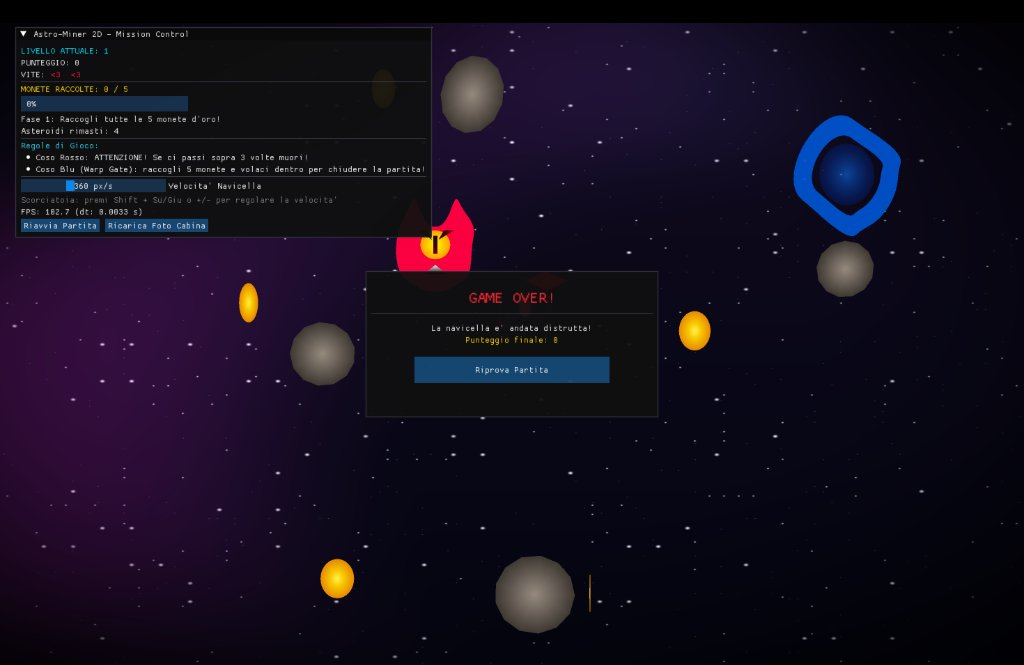
\includegraphics[width=0.76\linewidth]{../../assets/screenshots/screenshot_gameover.jpg}
    \caption{Banner modale di Game Over centrato con pivot $(0.5, 0.5)$ e visualizzazione del punteggio finale.}
\end{figure}

% ==============================================================================
\section{Compilazione, Avvio Rapido e Conclusioni}
% ==============================================================================
Il repository \texttt{proj-2D/} è interamente autosufficiente grazie all'inclusione statica delle librerie in \texttt{external/}:
\begin{itemize}
    \item \textbf{Avvio rapido (doppio click):} \texttt{AstroMiner.app} o \texttt{Avvia\_AstroMiner.command} su macOS;\\ \texttt{Avvia\_AstroMiner.bat} su Windows.
    \item \textbf{Build manuale da terminale (CMake):} \texttt{cmake -B build \&\& cmake --build build} ed esecuzione di \texttt{./build/Interactive2DWorld} (su Windows è possibile generare la soluzione Visual Studio 2022 \texttt{.sln} con \texttt{-G "Visual Studio 17 2022" -A x64}).
\end{itemize}
\noindent In conclusione, l'elaborato integra in un'unica architettura C++17 / OpenGL 3.3 Core Profile modulare i principi fondamentali della grafica 2D programmabile: trasformazioni gerarchiche, curve interpolanti di Hermite $C^1$, buffer sharing statico, shader procedurali in NDC, collisioni analitiche e simulazione fisica indipendente dal frame rate.

\end{document}
